\chapter[EMERGENCY]{EMERGENCY PROCEDURES}
\thumbtab{Em Proc}{1}
\localtableofcontents
\thispagestyle{plain}
\cleardoublepage

\marginfigeometry

\section{TAKEOFF}

\section{IN-FLIGHT}

\clearpage

\section{LANDING}

\marginfigrestore

\subsection{FLAMEOUT LANDING}

\begin{tcoloritemize}
    \blueitem[Energy \break Management]
    Engine flameout means that the aircraft is now operating with a fixed total energy,
    which must be used carefully

    \medskip
    If you are reading this for the first time following a flameout, 
    it's too late, eject now.

    \blueitem[Optimal Airspeed]
    \textbf{LG Up} --- 200 kts
    
    \medskip
    \textbf{LG Down} --- 190 kts
    
    \bigskip
    Increase by 5 kts for every 1000 lbs of fuel / stores

    \blueitem[Optimal AOA]
    \textbf{LG Up} --- 7 deg AOA achieves optimal airspeed

    \blueitem[Glideslope] Maximum range glideslope
    approx. 7nm per 5000 ft AGL with gear up,
    7 deg AOA, no stores retained

    \blueitem[Bank Angle]
    To minimize altitude loss in turns bank at
    
    \medskip
    \textbf{LG Up} --- 50 deg

    \medskip
    \textbf{LG Down} --- 55 deg
\end{tcoloritemize}

\subsubsection{OVERHEAD APPROACH}

\begin{tcoloritemize}
    \blueitem[Approach \break Pattern]
    Reference \cref{fig:proc_em:landing:flameout:overhead}, 
    if overhead pattern key positions cannot be reached use a straight-in 
    described in \cref{subsec:proc_em:landing:flameout:straightin}

    \blueitem[A \quad High Key]
    \textbf{Location} --- approx {1/3 down down the runway} from desired touchdown point

    \bigskip
    \textbf{Altitude} --- {7'000-10'000 ft AGL},
    recommend 7'000 ft plus 500 ft for every 1'000 lbs of fuel/stores

    \blueitem[B \quad Low Key]
    \textbf{Location} --- {1 nm abeam} point of rollout for final 

    \bigskip
    \textbf{Altitude} --- {3'000-5'000 ft AGL},
    recommend 3'000 ft plus 250 ft for every 1'000 lbs of fuel/stores

    \blueitem[C \quad Base Key]
    \textbf{Location} --- midpoint of final turn from downwind to final,
    {1.25 nm from touchdown point}

    \bigskip
    \textbf{Altitude} --- {2'000 ft AGL minimum}
\end{tcoloritemize}

\notebox{
    \begin{itemize}
        \item EPU consumes approx 15\% EPU fuel per minute
        \item JFS reduces EPU load, conserving fuel
    \end{itemize}
}

\begin{figure}[htbp]
    \centering
    \begin{subfigure}[t]{\linewidth}
        \centering
        \begin{tikzpicture}[figstyle]

            % coordinates
            \coordinate (td_des) at (0,0);
            \coordinate (high_key) at (15,30);
            \coordinate (inter_high_low) at (30,25);
            \coordinate (low_key) at (-15,15);
            \coordinate (base_key) at (-30,8);
    
            % runway
            \fill[]
            ($(td_des)+(-5,0)$) 
            -- ($(td_des)+(45,0)$)
            -- ($(td_des)+(45,-0.5)$)
            -- ($(td_des)+(-5,-0.5)$)
            -- cycle;

            \foreach \n in {5, 10, 15, 20, 25} {
                \draw[thin]
                (\n,0) 
                -- ++(90:0.5)
                -- ++(0:3)
                -- ++(-90:0.5)
                -- cycle
                (\n+0.25,0) -- ++(90:0.5)
                (\n+2.75,0) -- ++(90:0.5);
            }

            \draw[thin]
            (9,0)
            -- ++(180:0.1)
            -- ++(90:1)
            -- ++(180:0.25)
            -- ++(90:0.25)
            -- ++(0:0.3)
            -- ++(90:0.5)
            -- ++(-90:0.5)
            -- ++(0:0.3)
            -- ++(-90:0.25)
            -- ++(180:0.25)
            -- ++(-90:1)
            -- cycle;
            
            % fighter
            \node[anchor=east] (fighter) at (high_key.west) {
                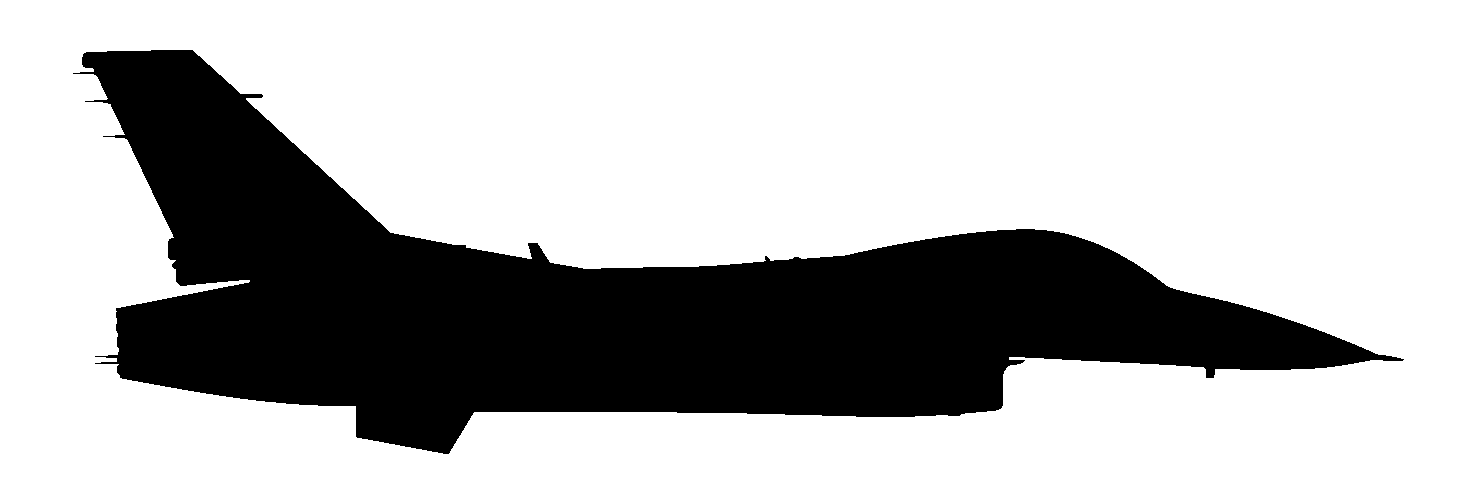
\includegraphics[
                    width=7.5mm,
                ]{diagrams/aircraft/silhouette_f16_side.pdf}
            };
    
            % approach
            \draw[->]
            (high_key)
            .. controls ($(high_key)+(-10:5)$) and ($(inter_high_low)+(90:4)$) ..
            (inter_high_low)
            .. controls ($(inter_high_low)+(-90:4)$) and ($(low_key)+(10:20)$) ..
            (low_key);
            \draw[->]
            (low_key)
            .. controls ($(low_key)+(190:10)$) and ($(base_key)+(60:1)$) ..
            (base_key);
            \draw[->]
            (base_key)
            .. controls ($(base_key)+(-60:10)$) and ($(td_des)+(177:5)$) ..
            (td_des);

            \node[red, font=\small\bfseries, above] at (high_key) {A};
            \node[red, font=\small\bfseries, above] at (low_key) {B};
            \node[red, font=\small\bfseries, left] at (base_key) {C};
            \node[red, font=\small\bfseries, below] at (td_des) {D};
    
            \filldraw[red] (high_key) circle (2pt);
            \filldraw[red] (low_key) circle (2pt);
            \filldraw[red] (base_key) circle (2pt);
            \filldraw[red] (td_des) circle (2pt);
        \end{tikzpicture}
        \caption{side view}
    \end{subfigure}

    \vspace{2em}
    \begin{subfigure}[t]{\linewidth}
        \centering
        \begin{tikzpicture}[figstyle]

            % coordinates
            \coordinate (td_des) at (0,0);
            \coordinate (high_key) at (15,0);

            % runway
            \draw[thick]
            ($(td_des)+(-5,-2)$) 
            -- ($(td_des)+(-5,2)$) 
            -- ($(td_des)+(45,2)$) 
            -- ($(td_des)+(45,-2)$) 
            -- cycle;
            \draw[thick]
            ($(td_des)+(-1,-1.33)$) -- ($(td_des)+(1,-1.33)$)
            ($(td_des)+(-1,-0.66)$) -- ($(td_des)+(1,-0.66)$)
            ($(td_des)+(-1,0.66)$) -- ($(td_des)+(1,0.66)$)
            ($(td_des)+(-1,1.33)$) -- ($(td_des)+(1,1.33)$);

            \draw[thick]
            (-5,2) 
            -- (-5,7)
            -- (4,7)
            -- (4,10)
            -- (29,10)
            -- (29,7)
            -- (45,7)
            -- (45,2)
            (-3,2)
            -- (-3,5)
            -- (10, 5)
            -- ++(0, -1)
            -- ++(-150:4)
            -- ++(2,0)
            -- ++(30:6)
            -- ++(3,0)
            -- ++(-30:6)
            -- ++(2,0)
            -- ++(150:4)
            -- ++(0,1)
            -- (43,5)
            -- (43,2);

            \draw[->]
            (high_key) 
            arc (90:-90:15)
            -- ++(-30,0) node (low_key) {};
            \draw[->]
            (low_key)
            arc(270:180:15) node (base_key) {};
            \draw[->]
            (base_key)
            arc (180:90:15)
            -- (td_des);

            % final markings
            \draw[<->, thin]
            (-15,10) -- (0,10) node[font=\small, pos=0.5, above] {0.75 nm};
            \draw[thin]
            (-15,0) -- ++(0,12)
            (0,0) -- ++(0,12);


            \node[red, font=\small\bfseries, below=2mm, anchor=north east]at (high_key) {A};
            \node[red, font=\small\bfseries, below] at (low_key) {B};
            \node[red, font=\small\bfseries, left] at (base_key) {C};
            \node[red, font=\small\bfseries, below=2mm] at (td_des) {D};

            \draw[<->, thin] (high_key) -- ++(0,-30) node[font=\small, pos=0.5] {1 nm};
            \draw[<->, thin] (base_key) -- (td_des) node[font=\small, pos=0.5, below right] {1.25 nm};

            \filldraw[red] (high_key) circle (2pt);
            \filldraw[red] (low_key) circle (2pt);
            \filldraw[red] (base_key) circle (2pt);
            \filldraw[red] (td_des) circle (2pt);
        \end{tikzpicture}
        \caption{top-down view}
    \end{subfigure}
    \caption{Flameout landing pattern --- overhead approach}
    \label{fig:proc_em:landing:flameout:overhead}
\end{figure}

% \begin{table}[htbp]
%     \centering
%     \small
%     \caption{Overhead approach parameters}
%     \begin{tabular}{l l r}
%         \toprule
%         \textbf{Point} & \textbf{Location} & \textbf{AGL } \\
%         \midrule
%         High Key & 1/3 along runway & 7-10'000 ft \\
%         Low Key & 1 nm abeam desired final rollout & 4-8'000 ft \\
%         Base Key & 1.25 nm from touchdown point & > 2000 ft \\
%         \bottomrule
%     \end{tabular}
% \end{table}

\clearpage

\subsubsection{STRAIGHT-IN APPROACH}
\label{subsec:proc_em:landing:flameout:straightin}

\begin{tcoloritemize}
    \blueitem[Approach \break Pattern]
    Reference \cref{fig:proc_em:landing:flameout:straightin}

    \blueitem[Point A]
    \textbf{Distance} --- 8 nm 

    \medskip
    \textbf{Altitude} --- 7'000 ft AGL minimum

    \medskip
    \textbf{Minimum EPU Fuel} --- 45\%

    \bigskip
    Minimum altitude to arrive at 2000 ft AGL position following optimal LG up glideslope 

    \medskip

    Continue optimal glide until desired touchdown point
    11-17$^\circ$ below horizon, 
    then lower LG and obtain optimal LG down airspeed

    \blueitem[Point B]
    \textbf{Distance} --- 4 nm 

    \medskip
    \textbf{Altitude} --- 4'000-8'000 ft AGL

    \medskip
    \textbf{Minimum EPU Fuel} --- 20\%

    \bigskip
    Airspeed, LG as required

    \blueitem[Area C]
    \textbf{Distance} --- 0-4 nm, desired touchdown point greater than 17$^\circ$ below horizon

    \bigskip
    Normal straight-in approach not feasible. Options:
    \begin{itemize}
        \item delay LG lowering, plan overhead approach from below desired high key altitude
        \item delay LG lowering, plan modified flightpath to low key
        \item lower LG, open speedbrakes, dive to intercept straight-in approach
    \end{itemize}
\end{tcoloritemize}

\notebox{
    \begin{itemize}
        \item EPU consumes approx 15\% EPU fuel per minute
        \item JFS reduces EPU load, conserving fuel
    \end{itemize}
}

\begin{figure}[htbp]
    \centering
    \begin{tikzpicture}[figstyle]

        % coordinates
        \coordinate (td_des) at (0,0);
        \coordinate (high_key) at (7.5,20);
        \coordinate (inter_high_low) at (15,17.5);
        \coordinate (low_key) at (-7.5,10);
        \coordinate (base_key) at (-15,6);
        \coordinate (final) at (170:8);
        \coordinate (straightin_base) at ($(final)+(150:9)$);
        \coordinate (straightin_a) at (-80,20);
        \coordinate (straightin_b1) at (-60,20);
        \coordinate (straightin_b) at (-50,20);
        \coordinate (straightin_b2) at (-40,20);
        % runway
        \fill[]
        ($(td_des)+(-5,0)$) 
        -- ($(td_des)+(30,0)$)
        -- ($(td_des)+(30,-0.5)$)
        -- ($(td_des)+(-5,-0.5)$)
        -- cycle;

        \foreach \n in {5, 10, 15, 20} {
            \draw[thin]
            (\n,0) 
            -- ++(90:0.5)
            -- ++(0:3)
            -- ++(-90:0.5)
            -- cycle
            (\n+0.25,0) -- ++(90:0.5)
            (\n+2.75,0) -- ++(90:0.5);
        }

        \draw[thin]
        (9,0)
        -- ++(180:0.1)
        -- ++(90:1)
        -- ++(180:0.25)
        -- ++(90:0.25)
        -- ++(0:0.3)
        -- ++(90:0.5)
        -- ++(-90:0.5)
        -- ++(0:0.3)
        -- ++(-90:0.25)
        -- ++(180:0.25)
        -- ++(-90:1)
        -- cycle;

        % overhead
        \draw[thin]
        (high_key)
        .. controls ($(high_key)+(0:3)$) and ($(inter_high_low)+(90:2)$) ..
        (inter_high_low)
        .. controls ($(inter_high_low)+(-90:4)$) and ($(low_key)+(10:10)$) ..
        (low_key)
        .. controls ($(low_key)+(190:5)$) and ($(base_key)+(90:2)$) ..
        (base_key)
        .. controls ($(base_key)+(-90:3)$) and ($(final)+(170:2.5)$) ..
        (final) -- (td_des);

        % fighter
        \node[anchor=south east] (fighter) at (straightin_a.west) {
            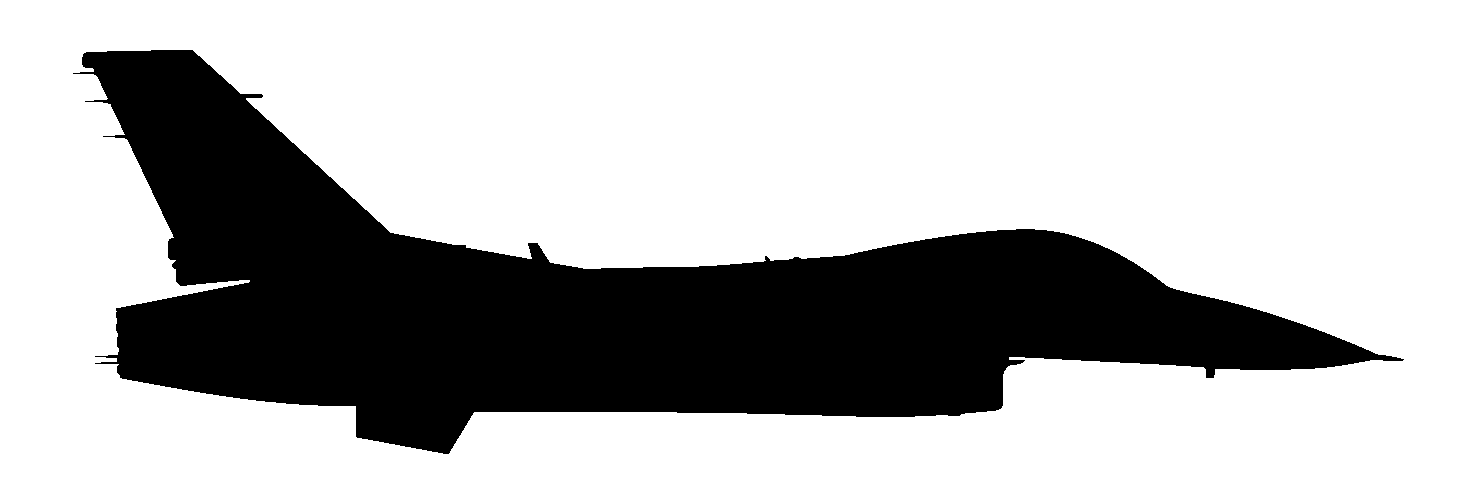
\includegraphics[
                width=7.5mm,
            ]{diagrams/aircraft/silhouette_f16_side.pdf}
        };

        \draw[thin]
        (straightin_a) -- (high_key) -- (30,20)
        (-80,0) -- (td_des);
            
        \draw[->]
        (straightin_a) -- (straightin_base) -- (final) -- (td_des)
        (straightin_b) -- (straightin_base) -- (final) -- (td_des);

        \draw[thin, dashed]
        (straightin_b1) -- (td_des) node[font=\footnotesize, pos=0, above] {11$^\circ$}
        (straightin_b2) -- (td_des) node[font=\footnotesize, pos=0, above] {17$^\circ$}
        (straightin_a) -- (td_des)node[font=\footnotesize, pos=0.10, below] {8$^\circ$};

        \draw[<->, thin]
        (24,20) -- ++(0,-20) node[font=\small, pos=1, below] {7'000 ft};

        \draw[thin]
        (straightin_a) -- ++(0,-20) node[font=\small, pos=1, below] {8 nm}
        (straightin_b1) -- ++(0,-20) node[font=\small, pos=1, below] {6 nm}
        (straightin_b2) -- ++(0,-20) node[font=\small, pos=1, below] {4 nm};
        
        \draw[thin]
        let \p1=(straightin_base) in 
        (straightin_base) -- (10,\y1);
        \draw[<->, thin]
        let \p1=(straightin_base) in 
        (3, \y1) -- (3,0) node[font=\small, pos=1, below] {2'000 ft};

        \node[red, font=\small\bfseries, above] at (straightin_a) {A};
        \node[red, font=\small\bfseries, above] at (straightin_b) {B};
        \filldraw[red] (straightin_a) circle (2pt);
        \filldraw[red] (straightin_b) circle (2pt);
        \filldraw[red] (td_des) circle (2pt);
        \path (-40,20) -- (high_key) node[red, font=\small\bfseries, pos=0.5, above] {C};

        \node[red, font=\footnotesize\bfseries, above, align=left, anchor=south west] at (high_key) {Overhead \\ Approach};
        \filldraw[red] (high_key) circle (2pt);

    \end{tikzpicture}
    \caption{Flameout landing pattern --- straight-in approach}
    \label{fig:proc_em:landing:flameout:straightin}
\end{figure}

% \begin{table}[htbp]
%     \centering
%     \small
%     \caption{Straight-in approach parameters}
%     \begin{tabular}{l r r r r}
%         \toprule
%         \textbf{Point} & \textbf{Range} & \textbf{Angle} & \textbf{AGL} & \textbf{EPU} \\
%         \midrule
%         A & 8 nm & 8$^\circ$ & 7'000 ft & > 45\% \\
%         B & 4 nm & 11-17$^\circ$ & 4-8'000 ft & > 20\% \\
%         C & < 4 nm & > 17$^\circ$ & --- & --- \\
%         \bottomrule
%     \end{tabular}
% \end{table}

\marginfigeometry

\subsubsection{PROCEDURE}

\begin{checklistenumerate}[start=0]
    \blueitem[Select Approach]

    Turn towards suitable runway, 
    accomplish overhead or straight-in approach
    \begin{itemize}
        \item Overhead approach altitudes
        \begin{itemize}
            \item \textbf{High Key --- 7'000-10'000 ft AGL} \\
            7'000 ft plus 500 ft per 1000 lbs of fuel / stores
            \item \textbf{Low Key --- 3'000-5'000 ft AGL}\\
            3'000 ft plus 250 ft per 1000 lbs of fuel / stores
        \end{itemize}
        \item Straight-in approach altitudes
        \begin{itemize}
            \item \textbf{8 nm --- 7'000 ft AGL}\\
            for optimal LG up glideslope until 2'000 ft AGL
            \item \textbf{4 nm --- 4'000-8'000 ft AGL}\\
            Lower LG once desired touchdown point 11-17$^\circ$ below horizon
        \end{itemize}
    \end{itemize}
    \blueitem[Stores]\dotfill \textbf{Jettison}\\
    \hfill(if required)
    \blueitem[Airspeed]\dotfill 200 kts
    \begin{itemize}
        \item increase speed 5 kts every 1000 lbs of fuel/stores
    \end{itemize}
    \blueitem[EPU]\dotfill \textbf{ON}
    \blueitem[JFS Switch]\dotfill \textbf{START 2}\\
    \hfill(below 20'000 ft MSL, 400 kts)
    \blueitem[AIR SOURCE Knob]\dotfill \textbf{RAM}\\
    \hfill(below 25'000 ft MSL)
    \blueitem[LG Handle]\dotfill \textbf{DN}
    \blueitem[ALT GEAR Handle]\dotfill Pull\\
    \hfill(if required)
    \blueitem[Airspeed]\dotfill 190 kts in pattern
\end{checklistenumerate}
\textbf{After Touchdown}
\begin{checklistenumerate}[resume]
    \blueitem[DRAG CHUTE Switch]\dotfill \textbf{DEPLOY}\\
    \hfill(if required)
    \blueitem[HOOK Switch]\dotfill \textbf{DN}\\
    \hfill(if required)
\end{checklistenumerate}

\clearpage

\marginfigrestore